\documentclass[10pt]{myarticle}

\usepackage{mlbasemath}
\usepackage{mlcomplessita}
\usepackage{pgfplots}
\usepackage{pgfplotstable}
\pgfplotsset{compat=1.5}
\usetikzlibrary{shapes,arrows,positioning,automata}

\usepackage[backend=bibtex]{biblatex}
\bibliography{multicore}

\author{Michele Laurenti}

\begin{document}

\title{Secondo homework}
\maketitle

\section{Scelte di implementazione}

Ho scelto di realizzare l'homework usando le immagini di OpenCL dopo essermi documentato al riguardo per realizzare l'esercizio dato in preparazione dell'esonero.
Per aprire le immagini ho utilizzato, su consiglio di un compagno di corso, la libreria di Sean T. Barrett\footnote{\url{https://github.com/nothings/stb}}, in grado di aprire buona parte delle immagini \code{jpeg} e \code{png} in circolazione e di salvare in formato \code{png}.
Ho sfruttato anche la piccola libreria fornita con la traccia dell'homework per aprire e salvare immagini \code{pgm}.

Ho usato alcune funzioni dalla libreria del laboratorio di Model Checking del prof. Tronci\footnote{\url{https://bitbucket.org/mclab/mclabutils}}.

Per impostare la dimensione del filtro e del work group nelle implementazioni locali ho utilizzato direttive di \code{define} fornite a \code{clBuildProgram}.
In questo modo posso allocare staticamente sul kernel array di dimensione opportuna. 

\subsection{Immagini in OpenCL}

In OpenCL un tipo di memory object \`e dedicato alla codifica di immagini.
Le immagini in OpenCL, oltre a godere di un grande insieme di ottimizzazioni invisibili al programmatore, sfruttano i tipi vettoriali di OpenCL C (e quindi l'architettura SIMD delle GPU) e sono manipolabili tramite un insieme di funzioni intuitive.
Utilizzare immagini permette di scrivere il kernel una sola volta, e vederlo funzionare con ogni tipo di immagine.

Indipendentemente dal numero di canali dell'immagine, ciascun pixel \`e sempre una quaterna \code{(r,g,b,a)}, codificata in un vettore di tipo \code{int}, \code{unsigned int} o \code{float}.
Immagini monocromatiche avranno come valore dei pixel sempre \code{(r,0,0,1)}.

Entrambe le librerie utilizzate trasferiscono le immagini in memoria in un array di \code{unsigned char} di dimensione $\code{width} \times \code{height} \times \code{\#\_of\_components}$.
La versione di OpenCL disponibile sul mio computer (1.2) non permette di copiare immagini da un formato a un altro\footnote{Dalla documentazione di OpenCL 1.2: ``It is currently a requirement that the \code{src\_image} and \code{dst\_image} image memory objects for \code{clEnqueueCopyImage} must have the exact same image format''.}.
Queste caratteristiche hanno forzato la scelta di \code{CL\_UNSIGNED\_INT8} come \emph{channel data type}, e nel kernel vengono quindi manipolati vettori \code{uint4}.

Sul computer su cui ho testato l'homework il \emph{channel order} \code{CL\_RGB} non \`e supportato assieme al \emph{channel data type} \code{CL\_UNSIGNED\_INT8} (utilizzato dalle librerie scelte per la lettura e scrittura di immagini).
I \emph{channel orders} scelti sono quindi \code{CL\_R} per immagini monocromatiche e \code{CL\_RGBA} per immagini a colori (con canale alpha sempre al massimo).

L'accesso alle immagini all'interno di un kernel \`e regolato da un \code{sampler}, un oggetto che permette di stabilire, fra le altre cose, cosa ritorner\`a un accesso a un pixel fuori dall'immagine: un'immagine specchiata, il pixel pi\`u vicino al bordo, un pixel nero, etc.
Un sampler permette di non preoccuparsi degli accessi fuori dall'immagine sorgente, se avvengono.

Non \`e possibile leggere e scrivere su una stessa immagine all'interno di un kernel OpenCL, ossia ogni immagine \`e o \code{read\_only} o \code{write\_only}.

\section{Prima implementazione}

Per un'immagine di dimensione $w \times h$, a cui va applicato un filtro di lato $f$, eseguo un kernel con NDRange $(w - f + 1) \times (h - f + 1)$.
La dimensione dell'immagine risultante sar\`a uguale a quella dell'NDRange.
Il kernel \`e immediato da scrivere: il work item $(x,y)$ legger\`a i valori dei pixel nel quadrato compreso fra $(x, y)$ e $(x + f - 1, y + f - 1)$ nell'immagine originale e ne calcoler\`a la media seguendo la matrice filtro fornitagli.
Il valore risultante andr\`a nel pixel $(x,y)$ dell'immagine filtrata.

Il sampler utilizzato ha \emph{addressing mode} impostato a \code{CL\_ADDRESS\_NONE}: non vengono fatti accessi fuori dai bordi dell'immagine.
Infatti il work item con indice globale $(0,0)$ acceder\`a ai pixel da $(0,0)$ a $(f-1,f-1)$, mentre il work item con indice globale $(w-f, h-f)$ acceder\`a ai pixel da $(w-f,h-f)$ a $(w-1,h-1)$.

Il codice della prima implementazione \`e nella funzione \code{clut\_blurImage} nel file \code{homework\_utils.c}.
Il codice kernel \`e nella funzione \code{blurImage} nel file \code{homework\_global.cl}.
Gli eseguibili \code{homework\_cpu} e \code{homework\_global} usano la prima implementazione.

\section{Prima ottimizzazione locale}

Per tentare di sfruttare la memoria locale, dato un filtro di lato $f$, la prima idea \`e di creare un buffer di dimensione $(w_{wg} + f - 1) \times (h_{wg} + f - 1)$ in cui i work item di un work group porteranno l'area di immagine di cui avranno bisogno.
Ciascun work item calcola il valore del proprio pixel nell'immagine risultante usando il buffer locale.

Per portare i pixel nel buffer, lo divido in sezioni grandi quanto il work group.
Ciascun work item, per ogni sezione, porta un pixel nel buffer.

In questa implementazione l'NDRange del kernel deve essere un multiplo della dimensione del work group, ma \`e comunque possibile conoscere all'interno del kernel OpenCL la dimensione di un'immagine (tramite due funzioni, \code{get\_image\_width} e \code{get\_image\_height}), senza dover passare parametri al kernel.

Il sampler utilizzato ha \emph{addressing mode} impostato a \code{CL\_ADDRESS\_CLAMP}: accedere a pixel fuori dall'immagine ritorna un pixel nero.

Dopo aver portato in memoria locale un'area dell'immagine, assieme a eventuali pixel neri se il work group si trova vicino al bordo, ciascun work item sfrutta il suo indice locale e la memoria locale per calcolare il pixel sfocato dato dall'indice globale.
Prima di scrivere il risultato dell'applicazione del filtro, ciascun work item controlla che il proprio indice globale non sia fuori dall'immagine, evitando quindi situazioni limite.

Il codice della prima implementazione locale \`e nella funzione \code{clut\_blurImage\_local} nel file \code{homework\_utils.c}.
Il codice kernel \`e nella funzione \code{blurImage\_local} nel file \code{homework\_local.cl}.
L'eseguibile \code{homework\_local} usa la prima implementazione.

\subsection{Limiti dell'ottimizzazione}

\`E possibile che spostare in memoria locale un'area dell'immagine entri in conflitto con le ottimizzazioni che gi\`a compie OpenCL.
OpenCL ottimizza automaticamente l'accesso alle immagini, ad esempio riordinando i pixel per favorire gli accessi vicini (figura \ref{fig:opencl_image_optimization}).
``This sort of optimization is only possible transparently (and hence different optimizations can be performed on different architectures) if we offer the kernel programmer no guarantees about the relative locations of memory elements'' \cite[p.~114]{hetcomp}.

\begin{figure}[tbh]
	\centering
	\includegraphics[width=\columnwidth]{images/opencl-image-optimization.jpg}
	\caption{Una possibile ottimizzazione, da \cite[p.~115]{hetcomp}: riordinare i pixel per favorire la localit\`a spaziale.}
	\label{fig:opencl_image_optimization}
\end{figure}

Alcuni dei pixel portati in memoria locale non vengono utilizzati, come si vede in figura \ref{fig:pixel_unused}.
%Sono circa $2 \, \left( {f^2 - f } \right)$.
Fino al $50\%$ dei pixel possono venire sprecati in questo modo.

\begin{figure}[tbh]
	\centering
	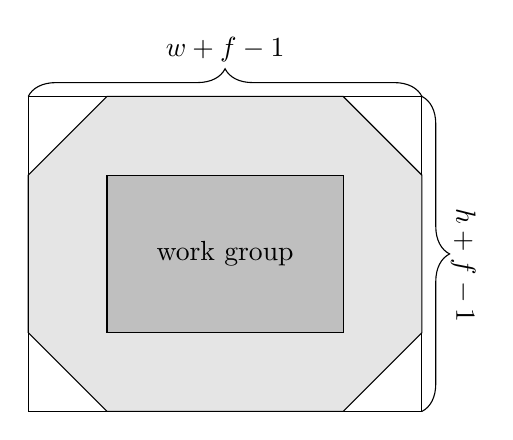
\begin{tikzpicture}
		\draw[black] (0,0) rectangle (5,4);
		\filldraw[fill = black!10!white, draw = black] 
		(1,0) -- (4,0) -- (5,1) -- (5,3) -- (4,4) -- (1,4) -- (0,3) -- (0,1) -- (1,0);
		\filldraw[fill = black!25!white, draw = black] (1,1) rectangle (4,3);
		\node[] at (2.5,2) {work group};
		\draw [decorate,decoration={brace,amplitude=10pt}]
		(5,4) -- (5,0) node [black,midway,label={[rotate=-90,yshift=0.4cm,xshift=-0.7cm]right:$h+f-1$}] {};
		\draw [decorate,decoration={brace,amplitude=10pt}]
		(0,4) -- (5,4) node [black,midway,yshift=0.6cm] {$w+f-1$};
	\end{tikzpicture}
	\caption{I pixel vicini al bordo non vengono utilizzati dal kernel.}
	\label{fig:pixel_unused}
\end{figure}

La versione locale non supporta tutte le dimensioni di filtro.
Il lato del work group dipende da tre fattori: il lato $f$ del filtro, la dimensione $N$ della memoria locale, e la dimensione massima $M$ di un work group.
Dobbiamo portare $(w_{wg} + f - 1) \times (h_{wg} + f - 1)$ pixel in memoria locale (ciascuno composto da 4 componenti, ciascuno di dimensione 4 byte).
Quindi deve valere $(w_{wg} + f - 1) \times (h_{wg} + f - 1) \cdot 16 \le N$.
Inoltre, $w_{wg} \times h_{wg}$ deve essere minore di $M$.
Utilizzo una funzione molto ingenua di dynamic programming per determinare la dimensione massima $w_{wg} \times h_{wg}$ del work group.

%\cite{hetcomp} consiglia come ottimizzazione l'allineamento degli accessi alla dimensione del bus di memoria.

\section{Seconda ottimizzazione locale}

I difetti maggiori della prima ottimizzazione sono due: la dimensione del filtro \`e limitata, e i work group diventano sempre pi\`u piccoli quando il filtro cresce oltre una certa grandezza.

Un'ottimizzazione migliore potrebbe essere mantenere la dimensione del work group fissa a $w_{wg} \times h_{wg}$, e portare in memoria locale l'area dell'immagine di cui il work group ha bisogno (grande sempre $(w_{wg} + f - 1) \times (h_{wg} + f - 1)$) un pezzo alla volta.

Divido l'area $(w_{wg} + f - 1) \times (h_{wg} + f - 1)$ di cui ho bisogno in sezioni grandi $w_{wg} \times h_{wg}$.
Porto in memoria locale ciascuna di queste sezioni una alla volta, con un doppio ciclo \code{for}, facendo copiare un pixel a work item.
Ciascun work item usa quindi i pixel di cui ha bisogno per calcolare la sfocatura prima di portare la sezione successiva in memoria locale.

Per capire quali pixel utilizzare per la sfocatura, ciascun work item determina gli indici iniziali e finali del quadrato di lato $f$ di cui ha bisogno nell'immagine originale.
Confrontando questi indici con gli indici di inizio e fine della sezione attualmente in memoria locale il work item stabilisce se alcuni di questi appartengono alla sezione.
Se \`e questo il caso, il work item determina la posizione rispetto al filtro dei pixel che ha a disposizione e calcola parte del risultato.

Questa implementazione non ha limiti alla dimensione del filtro, ma anche qui parte dei pixel portati in memoria locale non vengono utilizzati, come illustrato dalla figura \ref{fig:pixel_unused}.
Inoltre, con filtri di dimensione grande, una volta portata in memoria locale una sezione dell'immagine di cui il work group ha bisogno, alcuni work item potrebbero non lavorare, non necessitando di nessuno dei pixel nella sezione.

Il codice della prima implementazione locale \`e nella funzione \code{clut\_blurImage\_local\_unlimited} nel file \code{homework\_utils.c}.
Il codice kernel \`e nella funzione \code{blurImage\_unlimited} nel file \code{homework\_unlimited.cl}.
L'eseguibile \code{homework\_unlimited} usa la prima implementazione.

\section{Risultati ottenuti}

Ho testato il programma su un MacBook Air 13" del 2014 con processore i5\footnote{\url{http://ark.intel.com/products/75030/Intel-Core-i5-4260U-Processor-3M-Cache-up-to-2_70-GHz}} e scheda video integrata.

Alcune delle informazioni restituite da OpenCL:
\begin{verbatim}
Device type           CPU
Device name           Intel Core i5-4260U
Max clock frequency   1.40 GhZ
Max compute units     4
Max work group size   1024
OpenCL version        OpenCL 1.2 
OpenCL C version      OpenCL C 1.2 
Global memory size    8.00 GB
Local memory size     32.00 KB

= = = = = = = = = = = = = = = = = = = = =

Device type           GPU
Device name           HD Graphics 5000
Max clock frequency   1.00 GhZ
Max compute units     40
Max work group size   512
OpenCL version        OpenCL 1.2 
OpenCL C version      OpenCL C 1.2 
Global memory size    1.50 GB
Local memory size     64.00 KB
\end{verbatim}

Considero come esecuzione ``seriale'' l'esecuzione della prima implementazione sulla CPU, e confronto i tempi di esecuzione con il programma sulla GPU e il programma ``ottimizzato'' sulla GPU.
L'esecuzione su CPU non \`e seriale, ma \`e comunque un buon parametro di confronto.
Nelle figure seguenti l'errore indicato rappresenta la massima differenza fra i tempi di esecuzione e il tempo di esecuzione medio per una data dimensione del filtro.

I test sono stati eseguiti su un'unica immagine a colori\footnote{\url{https://www.flickr.com/photos/olivercharles/14550569782/sizes/k/}, jpeg di dimensione $2048 \times 1617$}.
La CPU del mio computer, con \emph{data type} \code{CL\_UNSIGNED\_INT8} (l'unico fornito dalle librerie), supporta solo immagini con \emph{channel order} \code{CL\_RGBA}.

Lo speedup fra CPU e GPU (figura \ref{fig:speedup_esecuzione}) con la prima implementazione \`e irregolare, ma in media \`e circa 9.
Nella figura \ref{fig:tempi_costanti} si vede che esecuzioni fatte a distanza di tempo dell'implementazione globale danno gli stessi tempi di esecuzione.

\begin{figure}[tbh]
\centering
\resizebox{\columnwidth}{!}{
	\begin{tikzpicture}
		\begin{axis}[
			scale only axis,
			width=\columnwidth,
			ymajorgrids,
			xlabel={dimensione filtro},
			ylabel={tempo (s)},
			legend pos = north west,
        ]
%			\pgfplotstableread{local_digest.dat}{\localtable}
			\pgfplotstableread{tests/global_digest.dat}{\globaltable}
			\pgfplotstableread{tests/cpu_digest.dat}{\cputable}
			\addplot[mark=o,red,error bars/.cd,y dir=both,y explicit]
			 table[x=filter,y=value,y error=media]  {\globaltable};
			 \addlegendentry{Global}
%			\addplot[mark=o,blue,error bars/.cd,y dir=both,y explicit]
%			 table[x=filter,y=value,y error=media]  {\localtable};
%			 \addlegendentry{Local}
			\addplot[mark=o,green,error bars/.cd,y dir=both,y explicit]
			 table[x=filter,y=value,y error=media]  {\cputable};
			 \addlegendentry{CPU}
		\end{axis}
	\end{tikzpicture}
	}
	\caption{Tempo di esecuzione dell'algoritmo globale su CPU e su GPU.}
	\label{fig:tempi_esecuzione_cpu}
\end{figure}

\begin{figure}[tbh]
\centering
\resizebox{\columnwidth}{!}{
	\begin{tikzpicture}
		\begin{axis}[
			scale only axis,
			width=\columnwidth,
%			xtick=data,
			ymajorgrids,
			xlabel={dimensione filtro},
			ylabel={speedup},
			legend pos = north west,
        ]
%			\pgfplotstableread{local_speedup_digest.dat}{\localtable}
			\pgfplotstableread{tests/global_speedup_digest.dat}{\globaltable}
%			\pgfplotstableread{cpu_digest.dat}{\cputable}
			\addplot[mark=o,red,error bars/.cd,y dir=both,y explicit]
			 table[x=filter,y=speedup]  {\globaltable};
			 \addlegendentry{Global}
%			\addplot[mark=o,blue,error bars/.cd,y dir=both,y explicit]
%			 table[x=filter,y=speedup]  {\localtable};
%			 \addlegendentry{Local}
%			\addplot[mark=o,green,error bars/.cd,y dir=both,y explicit]
%			 table[x=filter,y=value,y error=media]  {\cputable};
%			 \addlegendentry{CPU}
		\end{axis}
	\end{tikzpicture}
	}
	\caption{Speedup dell'algoritmo globale da CPU a GPU.}
	\label{fig:speedup_esecuzione}
\end{figure}

\begin{figure}[tbh]
\centering
\resizebox{\columnwidth}{!}{
	\begin{tikzpicture}
		\begin{axis}[
			scale only axis,
			width=\columnwidth,
			ymajorgrids,
			xlabel={dimensione filtro},
			ylabel={tempo (s)},
			legend pos = north west,
        ]
			\pgfplotstableread{tests/global_digest.dat}{\localtable}
			\pgfplotstableread{tests/global_digest_old.dat}{\globaltable}
%			\pgfplotstableread{cpu_digest.dat}{\cputable}
			\addplot[mark=o,red,error bars/.cd,y dir=both,y explicit]
			 table[x=filter,y=value,y error=media]  {\globaltable};
			 \addlegendentry{Prima serie di test}
			\addplot[mark=o,blue,error bars/.cd,y dir=both,y explicit]
			 table[x=filter,y=value,y error=media]  {\localtable};
			 \addlegendentry{Seconda serie di test}
%			\addplot[mark=o,green,error bars/.cd,y dir=both,y explicit]
%			 table[x=filter,y=value,y error=media]  {\cputable};
%			 \addlegendentry{CPU}
		\end{axis}
	\end{tikzpicture}
	}
	\caption{Esecuzioni a distanza di tempo danno gli stessi risultati.}
	\label{fig:tempi_costanti}
\end{figure}

Il tempo di esecuzione dell'implementazione globale aumenta rispetto a filtri di dimensioni simili quando la dimensione del filtro \`e 31, 49, 53, 55, 63.
Evidentemente l'esecuzione 

Come si vede dalla figura \ref{fig:tempi_esecuzione}, le ottimizzazioni non sono esattamente tali: i tempi di esecuzione aumentano leggermente.
I tempi sono per\`o distribuiti pi\`u regolarmente.

Sul computer su cui ho effettuato i test la dimensione della memoria locale della GPU \`e 65536 ($2^{16}$) byte, e la dimensione massima di un work group \`e 512.
Per $f \le 43$ la dimensione del work group non varia.
Per $f > 43$, la dimensione del work group diminuisce gradualmente, e il tempo di esecuzione (che prima seguiva l'andamento dell'algoritmo globale) aumenta pi\`u rapidamente.

\begin{figure*}[tbh]
\centering
\resizebox{\textwidth}{!}{
	\begin{tikzpicture}
		\begin{axis}[
			scale only axis,
			width=\textwidth,
			ymajorgrids,
			xlabel={dimensione filtro},
			ylabel={tempo (s)},
			legend pos = north west,
        ]
			\pgfplotstableread{tests/local_digest.dat}{\localtable}
			\pgfplotstableread{tests/unlimited_digest.dat}{\unlimitedtable}
			\pgfplotstableread{tests/global_digest.dat}{\globaltable}
%			\pgfplotstableread{cpu_digest.dat}{\cputable}
			\addplot[mark=o,red,error bars/.cd,y dir=both,y explicit]
			 table[x=filter,y=value,y error=media]  {\globaltable};
			 \addlegendentry{Global}
			\addplot[mark=o,green,error bars/.cd,y dir=both,y explicit]
			 table[x=filter,y=value,y error=media]  {\localtable};
			 \addlegendentry{Local, I implementazione}
			\addplot[mark=o,blue,error bars/.cd,y dir=both,y explicit]
			 table[x=filter,y=value,y error=media]  {\unlimitedtable};
			 \addlegendentry{Local, II implementazione}
%			\addplot[mark=o,green,error bars/.cd,y dir=both,y explicit]
%			 table[x=filter,y=value,y error=media]  {\cputable};
%			 \addlegendentry{CPU}
		\end{axis}
	\end{tikzpicture}
	}
	\caption{Tempi di esecuzione dell'algoritmo globale e degli algoritmi locali su GPU.}
	\label{fig:tempi_esecuzione}
\end{figure*}

L'andamento del tempo di esecuzione con la seconda ottimizzazione \`e quadratico nella dimensione del filtro.

\section{Bug delle implementazioni}

Sul mio computer tutte e tre le implementazioni danno problemi per dimensioni del filtro troppo grandi.
L'esecuzione del kernel termina correttamente: la funzione \code{clGetEventInfo}, con argomenti l'evento legato al kernel e \code{CL\_EVENT\_COMMAND\_EXECUTION\_STATUS} ritorna \code{CL\_COMPLETE}, ma la funzione \code{clGetEventProfilingInfo} ritorna sempre 0 come \code{CL\_PROFILING\_COMMAND\_END}.
Tentare di leggere il contenuto dell'immagine dopo la terminazione del kernel causa un accesso a memoria non allocata, crashando il programma.

Sul mio computer l'implementazione globale d\`a problemi quando la dimensione del filtro \`e 67 o 83.
La prima implementazione locale d\`a problemi per dimensioni del filtro oltre il 55.
La seconda implementazione locale d\`a problemi per dimensioni del filtro vicine a 100.

Secondo \cite{nvidiakernel}, indicatomi da un compagno di corso, un kernel CUDA non pu\`o restare in esecuzione per pi\`u di 5 secondi\footnote{``What is the maximum kernel execution time?'' ``[...] individual GPU program launches have a maximum run time of around 5 seconds. [...] This is caused by the Windows `watchdog' timer that causes programs using the primary graphics adapter to time out if they run longer than the maximum allowed time.''} su una GPU Nvidia utilizzata anche dal display.
La FAQ \`e relativa a una scheda grafica di un altro produttore, a un'altra libreria e a un altro sistema operativo, ma \`e possibile che limitazioni di questo tipo siano presenti anche su computer Apple.
Non sono riuscito a trovare informazioni al riguardo.

Una soluzione \`e quella di spezzare l'esecuzione del kernel in pi\`u parti.
\`E sufficiente fornire gli argomenti al kernel una sola volta e eseguire pi\`u kernel con NDRange ridotti e offset impostato opportunamente.
Scegliere quando e come dividere l'NDRange originale in un certo numero di NDRange pi\`u piccoli \`e un problema non banale: dimensioni troppo piccole e non bilanciate con la dimensione del work group potrebbero non dare lavoro a tutti i work item.

Una soluzione pi\`u semplice \`e eseguire il kernel su una GPU dedicata.

\section{Immagini filtrate}

Alcuni esempi di applicazione del filtro sono in figura \ref{fig:applicazione_filtro}.
I primi due filtri sono stati applicati con l'implementazione globale, il terzo con la seconda implementazione locale.

\begin{figure*}[tbh]
	\centering
	\includegraphics[width=\columnwidth]{images/result-example-1.png}
	\includegraphics[width=\columnwidth]{images/result-example-9.png}
	\\
	\includegraphics[width=\columnwidth]{images/result-example-35.png}
	\includegraphics[width=\columnwidth]{images/result-example-89.png}
	\caption{Risultati dell'applicazione del filtro. Nell'ordine: immagine originale, filtro di dimensione 9, filtro di dimensione 35, filtro di dimensione 89.}
	\label{fig:applicazione_filtro}
\end{figure*}

\section{Eseguire il programma}

Questa \`e la struttura dei file nell'homework:
\begin{verbatim}
Makefile
homework_cpu.c
homework_global.c
homework_global.cl
homework_local.c
homework_local.cl
homework_unlimited.c
homework_unlimited.cl
homework_utils.c
homework_utils.h
mclabutils/
mlclut/
mlutils/
stb/
\end{verbatim}

La cartella \code{mclabutils} contiene i file essenziali della libreria di Model Checking del prof. Tronci.
La cartella \code{stb} contiene la libreria per l'apertura e la scrittura di immagini di Sean T. Barrett.
Le altre due cartelle contengono utility scritte da me.
La cartella \code{mlutils} contiene semplici utility in C, principalmente per l'apertura e la lettura di file riga per riga.
La cartella \code{mlclut} contiene utility per l'apertura di immagini in OpenCL, funzioni per stampare descrizioni di errori e costanti di OpenCL, e funzioni per creare e compilare programmi OpenCL o per ottenere platforms e devices.

Per compilare l'homework \`e sufficiente il comando \code{make all} nella cartella principale.
I programmi eseguibili sono quattro:
\begin{verbatim}
homework_global
homework_cpu
homework_local
homework_unlimited
\end{verbatim}

Tutti e quattro chiedono due parametri in input: il percorso dell'immagine a cui applicare il filtro e la dimensione del filtro.
Il codice di ritorno di tutti i programmi \`e 0 se il filtro viene applicato senza problemi e l'immagine risultante viene salvata correttamente, 1 altrimenti.

I primi due eseguibili producono l'immagine \code{output.png}, il terzo produce l'immagine \code{output\_local.png}, il quarto produce l'immagine \code{output\_unlimited.png}.

\renewcommand{\refname}{Riferimenti}

\printbibliography

\end{document}

